%%%%%%%%%%%%%%%%%%%%%%%%%%%%%%%%%%%%%%%%%%%%%%%%%%%
%                                                 %
%                     SECTION                     %
%                                                 %
%%%%%%%%%%%%%%%%%%%%%%%%%%%%%%%%%%%%%%%%%%%%%%%%%%%

\section*{Details}

Several modalities \cite{kopans2004breast} are used as an adjunct look modality for questionable situations where the breast of the patient has a life time risk. The images produced by the \textbf{Medical Imaging (MI)} exams are similar in acquisition, however the costs (time and money) are typically different. This behaviour is leading the \textbf{RR} workflow standards and methodology to remain scarce \cite{rawson2016lessons, saltzherr2013cost}, which give us little information to support a workflow validation through interviews and observations. Therefore, we will not assume a low-level workflow of the \textbf{RR} and will assume from now a high-level workflow, where the rules to trigger the acquisition of the several modalities are not specified.

\hfill

The following text can be used to motivate/introduce a final paper to write. So it's more or less like this:

%%%%%%%%%%%%%%%%%%%%%%%%%%%%%%%%%%%%%%%%%%%%%%%%%%%

\hfill

\begin{enumerate}

\item Mammography appears as the 1st imaging modality, and constitutes a screening exam. The reason is that the exam in this modality (X-Ray) has little cost.

\item It is begun to realise that not all the examinations (recognised) in mammography are conclusive. The main reason for this is the type of breast (Figure \ref{fig:workflow}). There are two types \cite{nothacker2009early, rhodes2011dedicated} of breasts: (1) adipose breasts (patterns A and B) and (2) dense breasts (patterns C and D). These types are leaving an international standard where mammography may not be sufficient in the diagnosis of a dense breast by concluding that this type of chest is opaque to the X-Ray. According to study was done, the dense breasts have 2X or 4X more likely to develop a tumour than the adipose breast.

\hfill

\textbf{Note:} supporting this international standard by the fact that there were cases where women unexpectedly possessed advanced tumours, although they did frequent X-Ray screenings.

\hfill

\item Therefore, it is necessary to have an additional examination, particularly in case of dense breast, in standards C and D (Figure \ref{fig:workflow}). Doing in these cases an ultrasound.

%%%%%%%%%%%%%%%%%%%%%%%%%%%%%%%%%%%%%%%%%%%%%%%%%%%

\hfill

\begin{figure}[h]
\centering
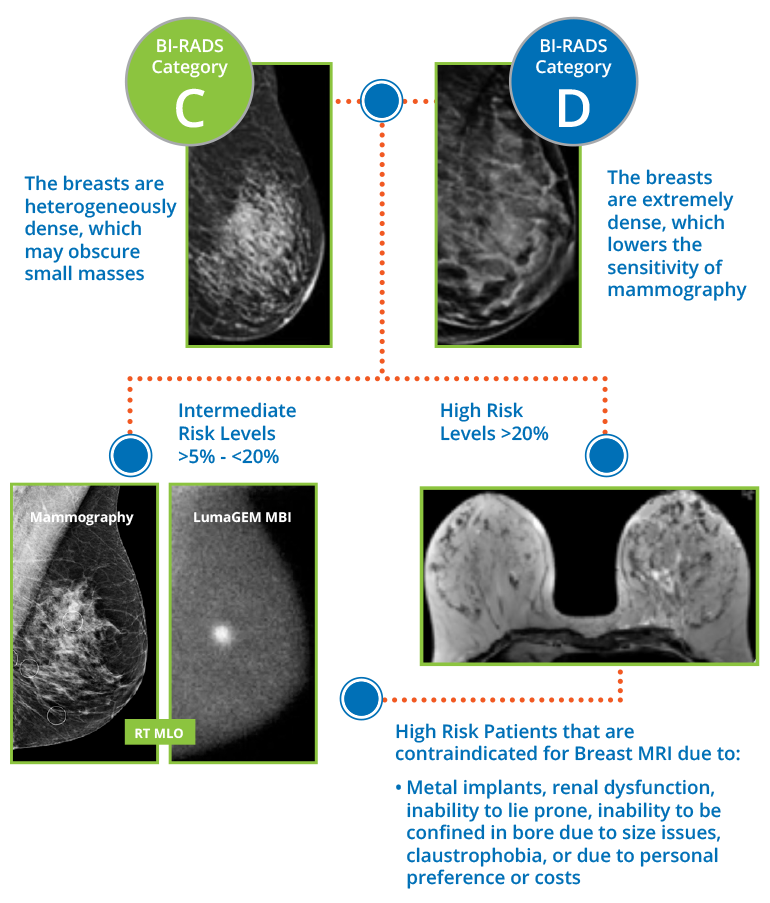
\includegraphics[width=0.75\textwidth]{workflow}
\caption{Workflow \cite{workflow}}
\label{fig:workflow}
\end{figure}

\hfill

%%%%%%%%%%%%%%%%%%%%%%%%%%%%%%%%%%%%%%%%%%%%%%%%%%%

\item There is not yet an international guideline (or standards) for elaborating MRI (which is a very expensive kind of exam). We proceed to this type of examination for women with family risk, the so-called BRCA1 and BRCA2 \cite{chen2007meta}. Being these mutations that the woman suffers, and being able to provoke a tumour (the case, for example, of Angelina Jolie).

\item In other cases (not mentioned in point 4) it is up to the radiologist to do MRI or not. It can happen, for instance, that on the palpation (performed by the radiologist) there are indications of tumour presence, without any suspicion in mammography. There you will advance to the MRI.

\item Still about point 5, there are cases where the patient is followed, and calcifications with suspected morphology are recorded (in mammography). In these situations, the radiologist advances to MRI.

\end{enumerate}

\hfill

%%%%%%%%%%%%%%%%%%%%%%%%%%%%%%%%%%%%%%%%%%%%%%%%%%%














%During several early preliminary meetings, we enter into a quest to understand the fundamental building blocks of our research into the Human-Computer Interaction (HCI) applied to Health Informatics (HI). In our research developments, we are doing a User-Centered Design (UCD) to develop a Medical Imaging (MI) system that will support a breast cancer diagnosis in multimodality of view. During the past months, we grew several pilot versions of the system improving it. However, by trying to solve it, we encounter some high-level issues regarding the user interaction. Those issues were encountered during our user tests on the Radiology Room since we were doing experiments with Clinicians, or more precisely with Radiologists.
%
%In this report, we will address several of the debated issues that are potential contributions to the scientific community. Also, this report is a baseline work for the Research and Doctoral developments of the author. During the time we had aggregate a set of questions that seem to be an essential list of items to have in mind and to answer during the time. The issues are as follow on the next record.
%
%\hfill
%
%List of questions that seem to be important to answer over the time:
%
%\hfill
%
%\begin{enumerate}
%\item What is already done between HCI and HI?
%\item How can we improve our system?
%\item Who can help us to achieve our goals?
%\end{enumerate}
%
%\hfill
%
%Although these questions seem to be vague, the questions are serving us as a contextualisation between research field and project relative topics. Both Figure \ref{fig:plan_1_2} and Figure \ref{fig:plan_3_4} are representing our meeting debate regarding the next resurgence of system-related issues.
%
%The first issue we debate (Figure \ref{fig:plan_1_2}) was related to the need of having a full number of \textit{annotators}. One of the suggestions from Professor Nuno Nunes was the strategy of trying to find a way of bringing non-medical experts to label our medical images. With a higher crowdsourcing workflow, we can extract a higher number of annotations from medical images. However, since the users are not medical experts we need to find a credible way to solve the domain issue. For instance, Professor Nuno Nunes gave us the example \cite{cao2016estimating} of his research work answering a similar problem/solution.
%
%%%%%%%%%%%%%%%%%%%%%%%%%%%%%%%%%%%%%%%%%%%%%%%%%%%%
%
%\hfill
%
%\begin{figure}[h]
%\centering
%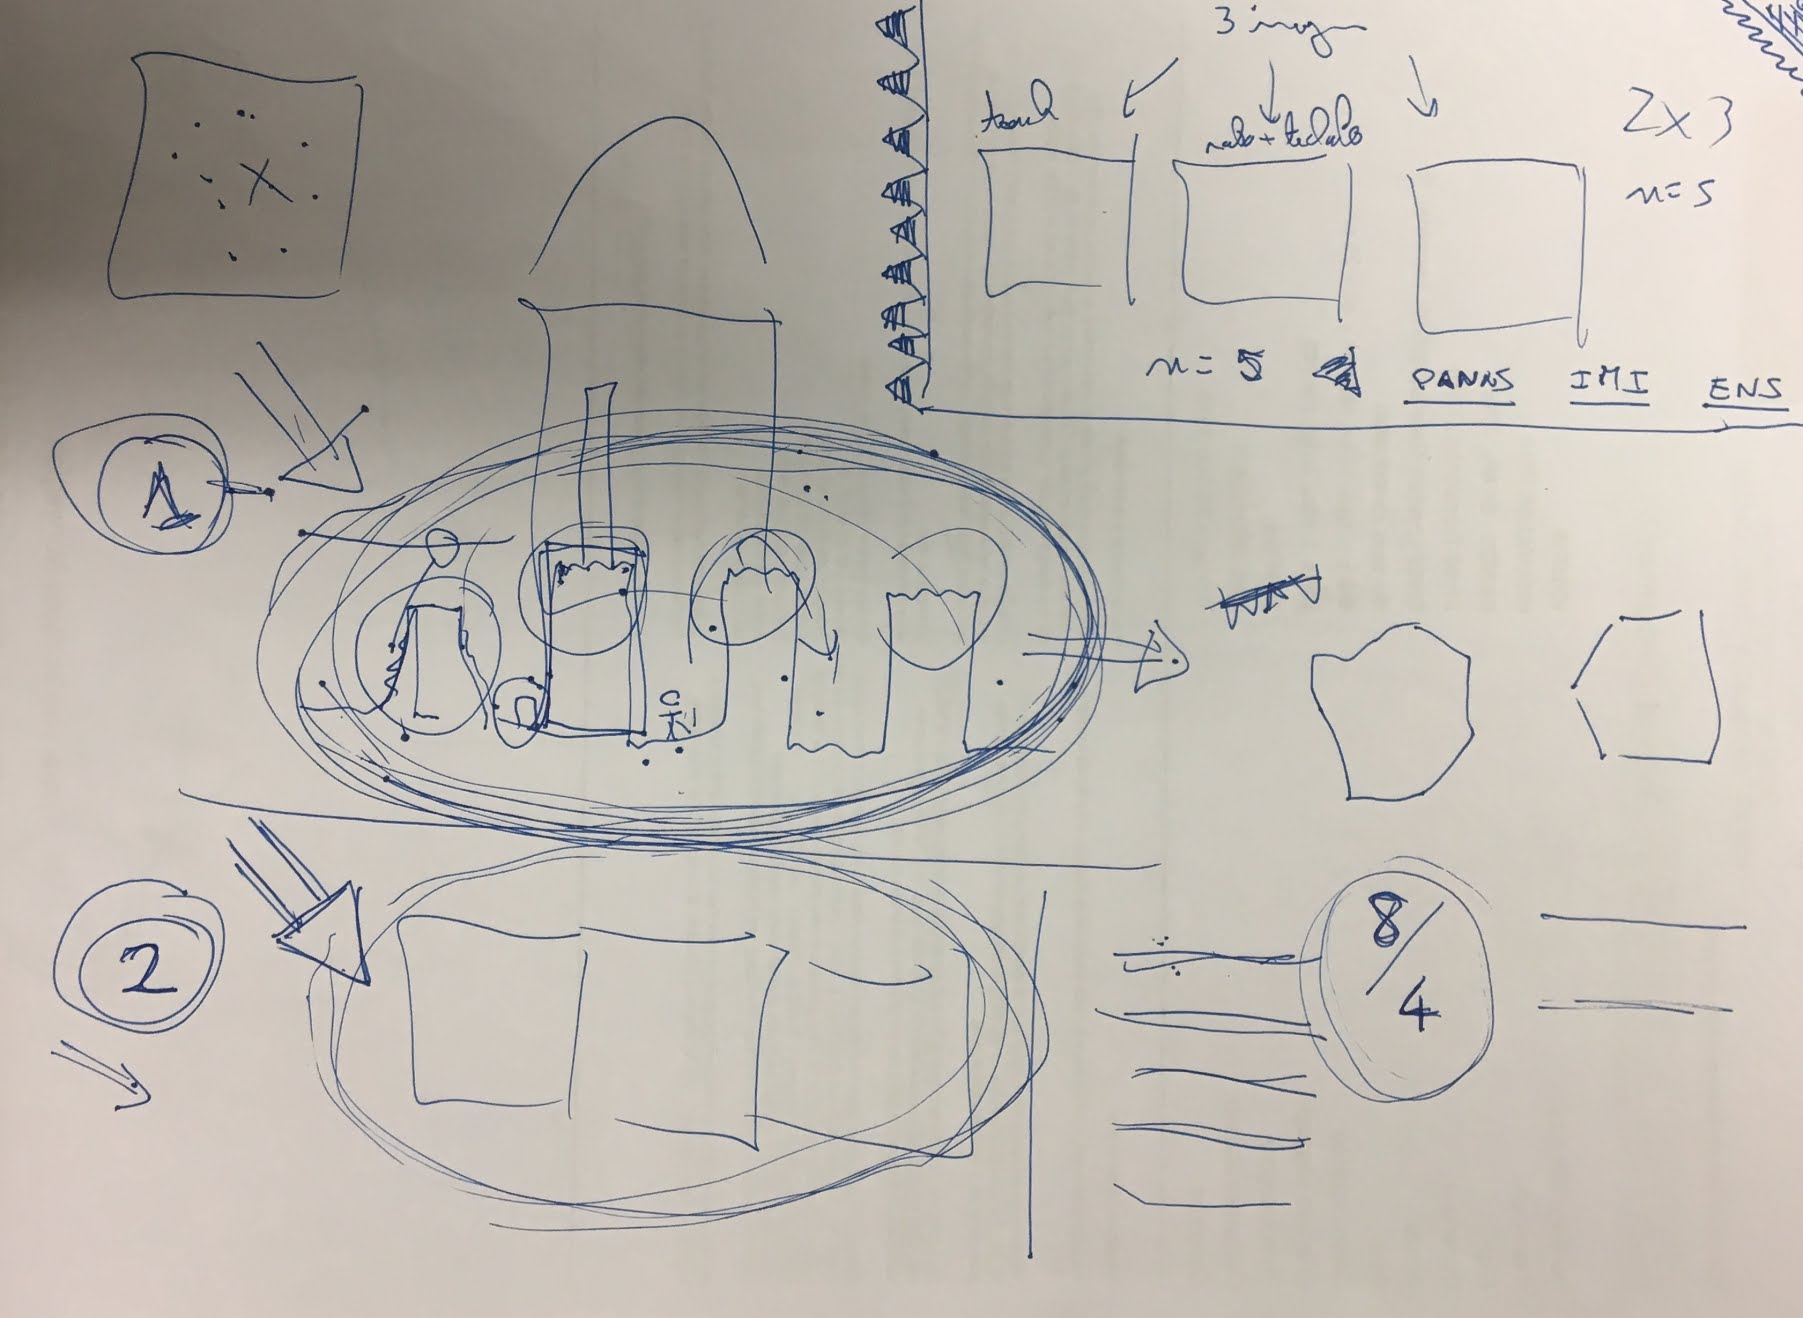
\includegraphics[width=0.75\textwidth]{plan_1_2}
%\caption{Plan 1}
%\label{fig:plan_1_2}
%\end{figure}
%
%\hfill
%
%%%%%%%%%%%%%%%%%%%%%%%%%%%%%%%%%%%%%%%%%%%%%%%%%%%%
%
%On the second issue (Figure \ref{fig:plan_1_2}), we discuss the opportunity of arguing our contribution as a multimodality related. The goal of this argument is to show, by giving evidence, that our multimodality of medical imaging is novel and bring to the healthcare systems a higher performance, as well as more accurate regarding the cancer diagnosis over medical imaging. For this issue we need to address and increase our network number of medical experts. At the moment we have between 8 to 12 medical experts, but we need at least 30 medical experts to cover our user tests.
%
%The next Figure \ref{fig:plan_3_4} covers what we debate regarding how to relate our novelties and compare the novel techniques (e.g. Figure \ref{fig:annotation_predictor_1}) with expected improvements by using new interaction techniques. The idea of Professor Nuno Nunes is to compare three different tasks with different interaction techniques each. The first one is the vanilla technique, where the user annotate the medical imaging with no system help. The second one is the technique the user receives recommendations for the next annotation point. Finally, the third one, the user press a region and the system automatically reproduce the annotation areas for that region. To test and validate this issue we need to measure performance and experience, comparing the three tasks and giving our conclusions.
%
%%%%%%%%%%%%%%%%%%%%%%%%%%%%%%%%%%%%%%%%%%%%%%%%%%%%
%
%\hfill
%
%\begin{figure}[h]
%\centering
%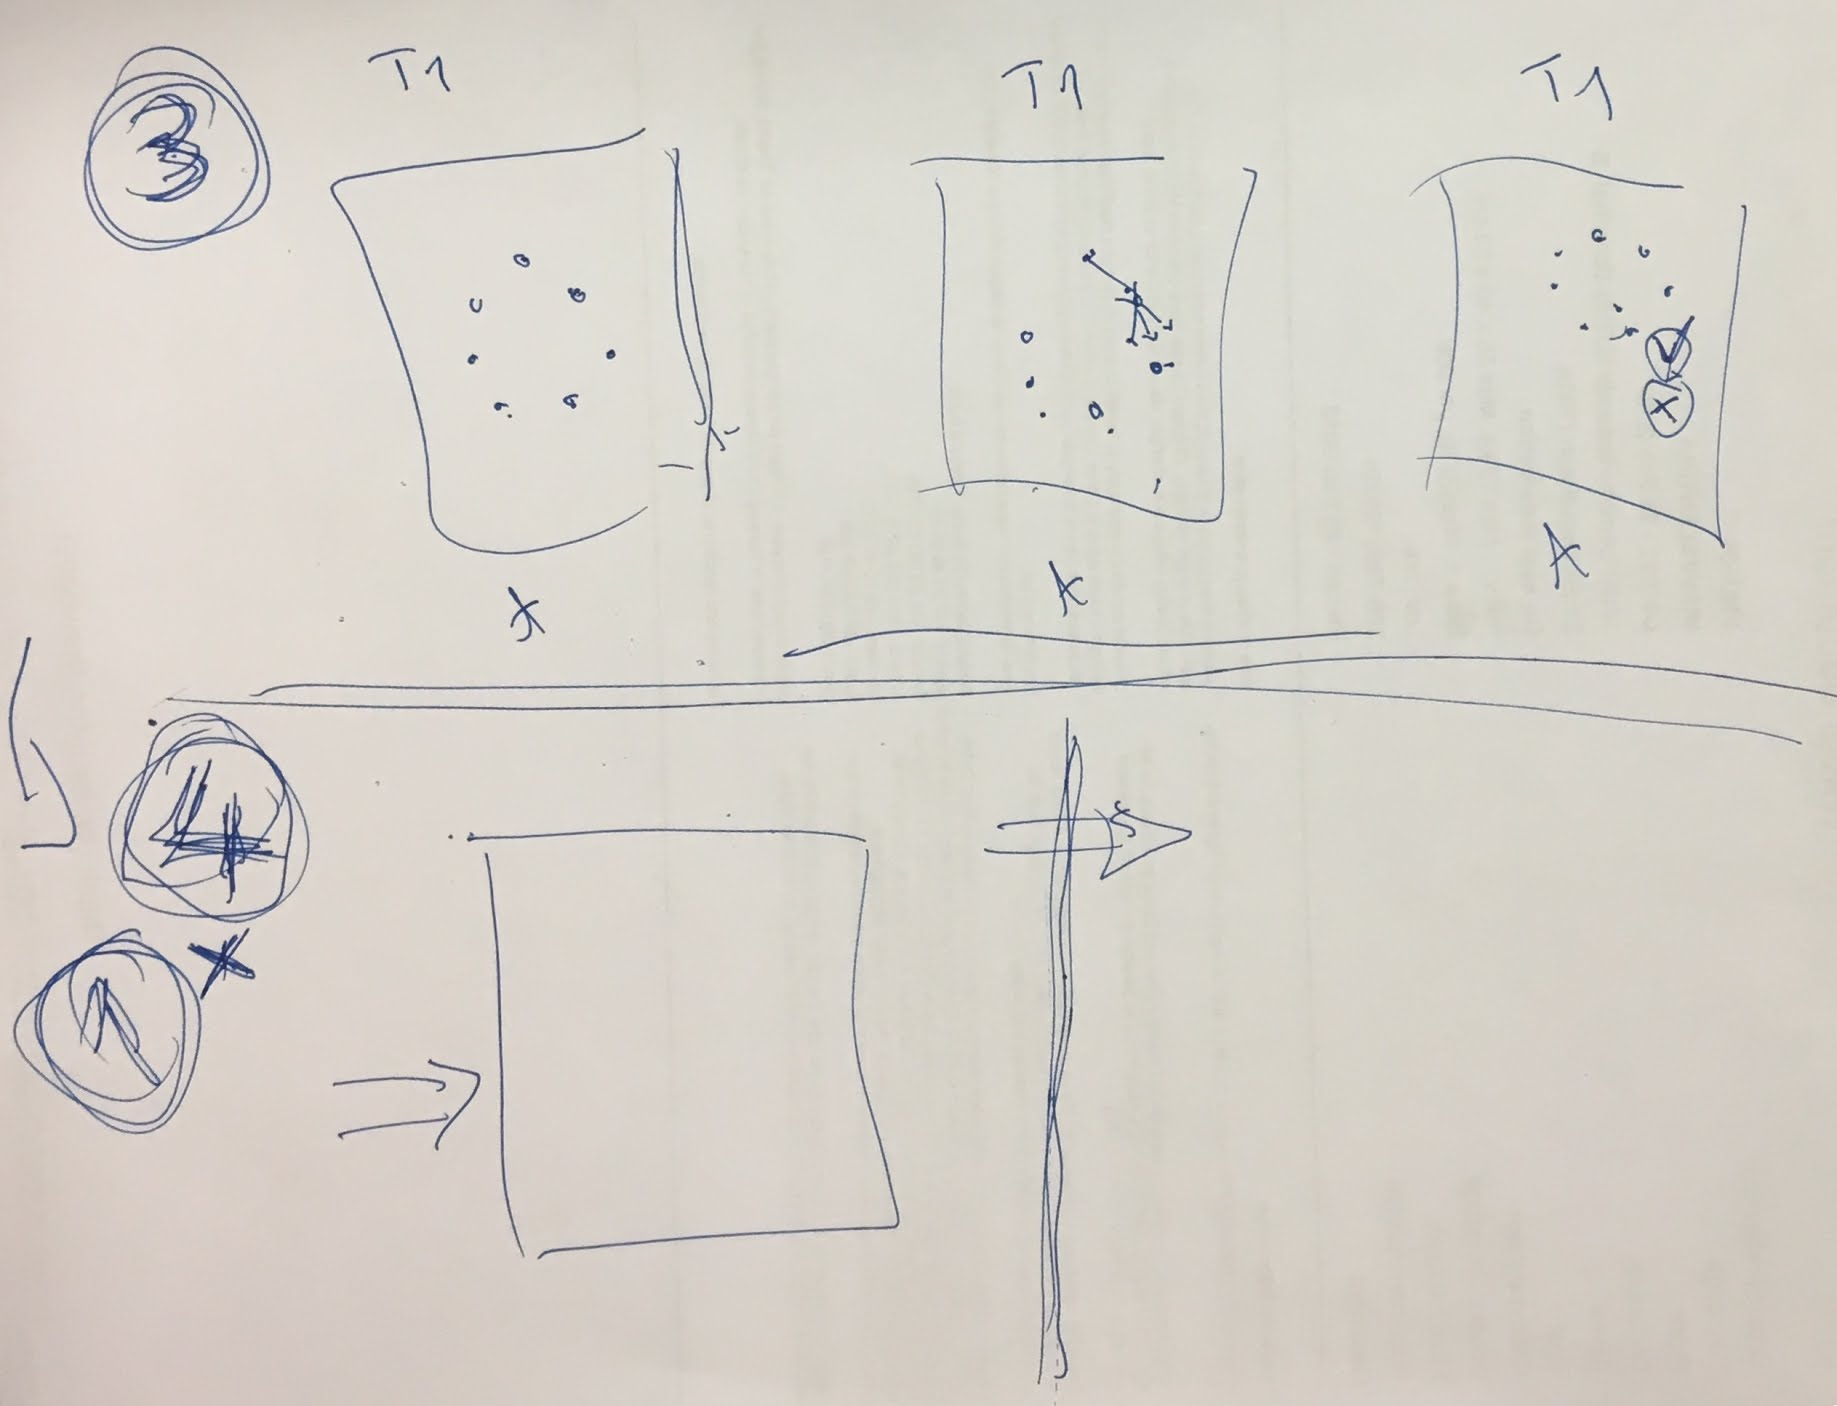
\includegraphics[width=0.75\textwidth]{plan_3_4}
%\caption{Plan 2}
%\label{fig:plan_3_4}
%\end{figure}
%
%\hfill
%
%%%%%%%%%%%%%%%%%%%%%%%%%%%%%%%%%%%%%%%%%%%%%%%%%%%%
%
%Last but not least, we debate a fourth issue (Figure \ref{fig:plan_3_4}) where it brings the first issue from Figure \ref{fig:plan_1_2}, where we bring together the idea of a crowdsourcing solution and test results of the novel interaction techniques with no medical experts. For this issue, it will be a more reliable test since we are testing again the methods where it reduces the need for experts. We are assuming here not being focused on labelling images, instead of it, we focus on improving interactions. Although we can also label images.
%
%Despite being a focus on high-level issues to solve in our system, we also have specific problems to solve. One of them is the problem of visualising stacks (Figure \ref{fig:rsvp_1}) of the \textbf{MRI} modality. When an image has a lesion, it is not easy to observe the wound and have a notion of the frames before and after the beginning and the end of that lesion. Therefore it is essential to give the user this notion of location. By studying a technique called \textit{RSVP}~\cite{brown2017role} we can address this issue more efficiently, while it is a potential and useful community contribution.
%
%%%%%%%%%%%%%%%%%%%%%%%%%%%%%%%%%%%%%%%%%%%%%%%%%%%%
%
%\hfill
%
%\begin{figure}[h]
%\centering
%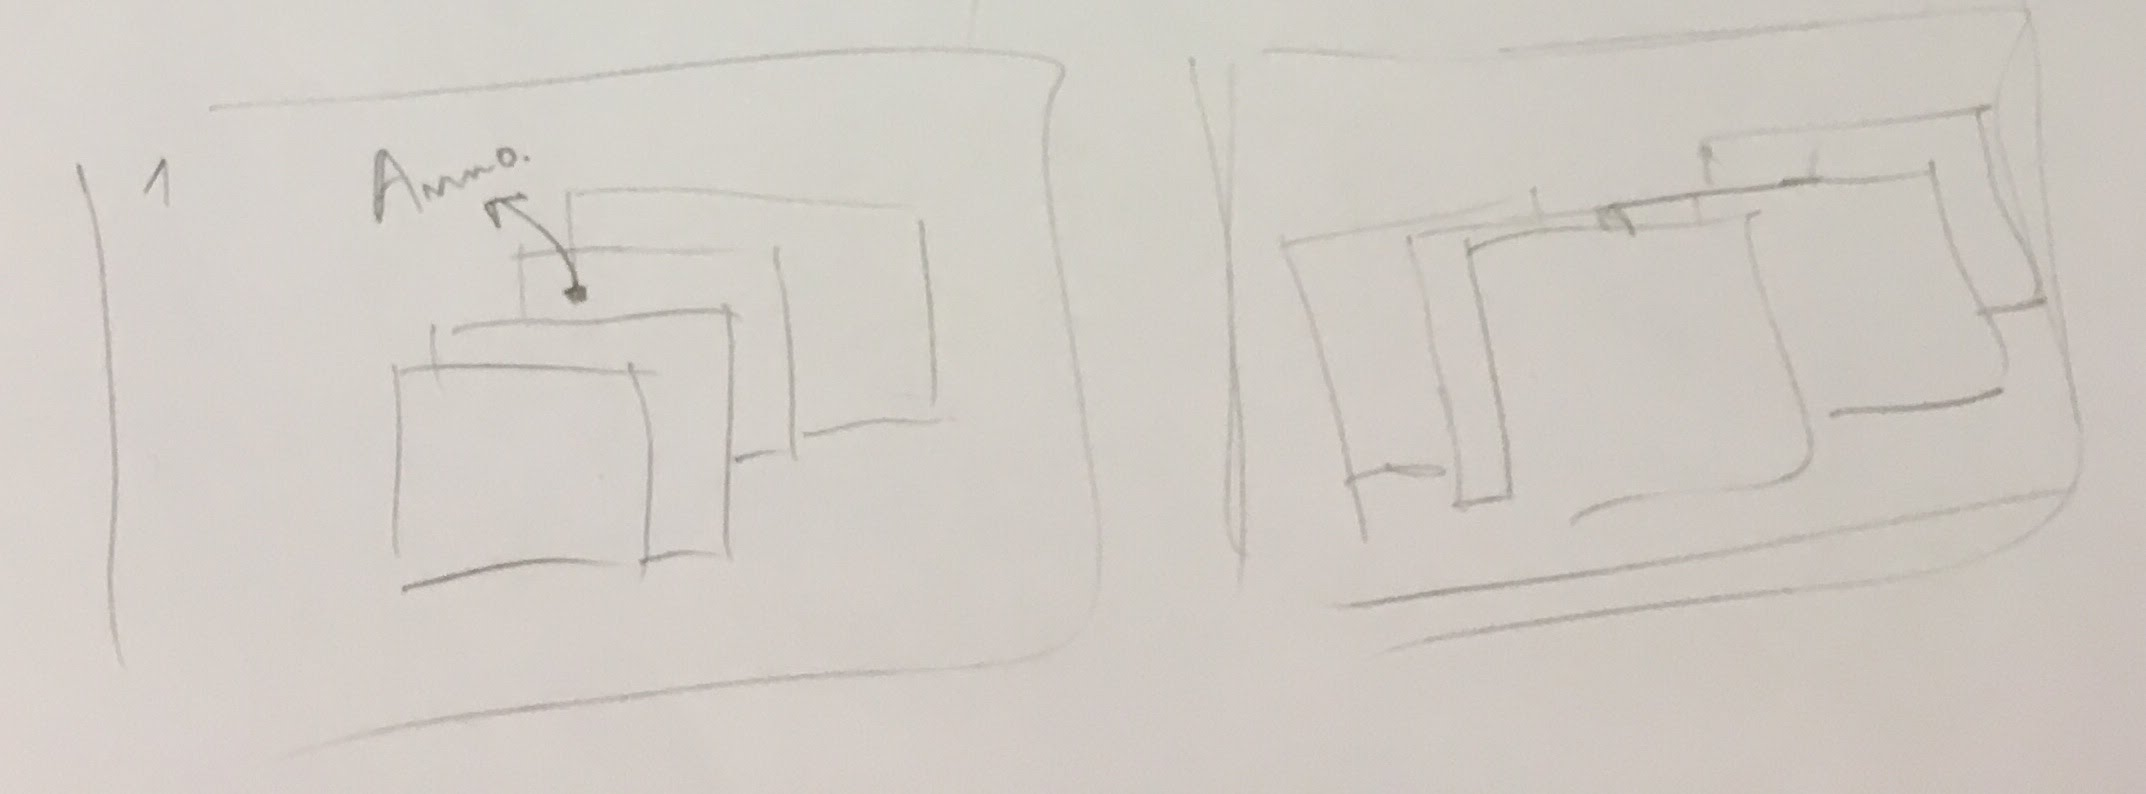
\includegraphics[width=0.75\textwidth]{rsvp_1}
%\caption{RSVP}
%\label{fig:rsvp_1}
%\end{figure}
%
%\hfill
%
%%%%%%%%%%%%%%%%%%%%%%%%%%%%%%%%%%%%%%%%%%%%%%%%%%%%
%
%%%%%%%%%%%%%%%%%%%%%%%%%%%%%%%%%%%%%%%%%%%%%%%%%%%%
%
%\hfill
%
%\begin{figure}[h]
%\centering
%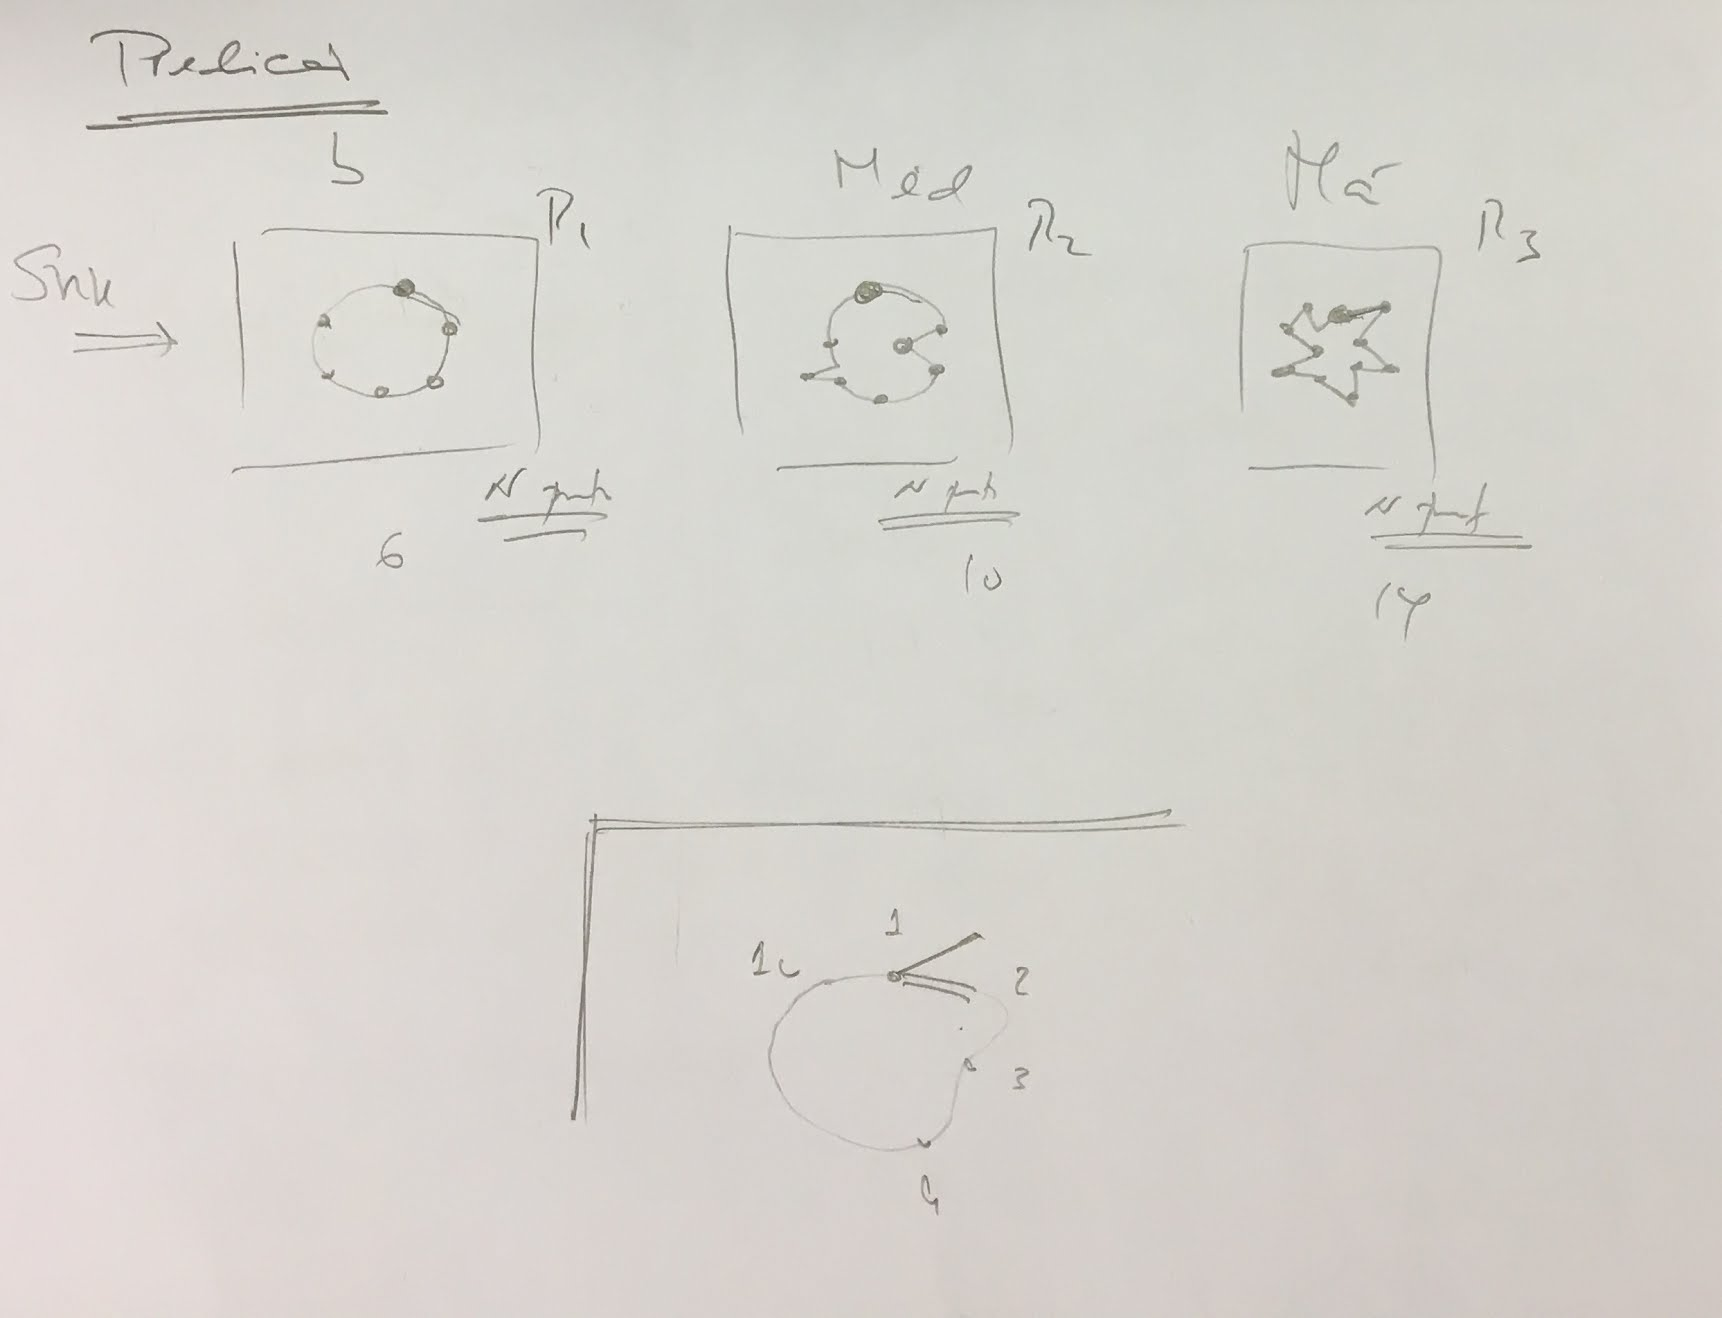
\includegraphics[width=0.60\textwidth]{annotation_predictor_1}
%\caption{Annotation Predictors Test}
%\label{fig:annotation_predictor_1}
%\end{figure}
%
%\hfill
%
%%%%%%%%%%%%%%%%%%%%%%%%%%%%%%%%%%%%%%%%%%%%%%%%%%%%
%
%Finally, we also address the predictors (Figure \ref{fig:annotation_predictor_1} and Figure \ref{fig:annotation_predictor_2}) issue. This issue is of chief interest since it has an immense contribution potential to the community. The idea of this solution is to simulate the presence of a recommendation system to recommend the next annotation point, simulating three different options. The simulation source come from an expert annotation on each image. We will compare three different images with three different difficulties. Than we show and simulate the system with other users.
%
%%%%%%%%%%%%%%%%%%%%%%%%%%%%%%%%%%%%%%%%%%%%%%%%%%%%
%
%\hfill
%
%\begin{figure}[h]
%\centering
%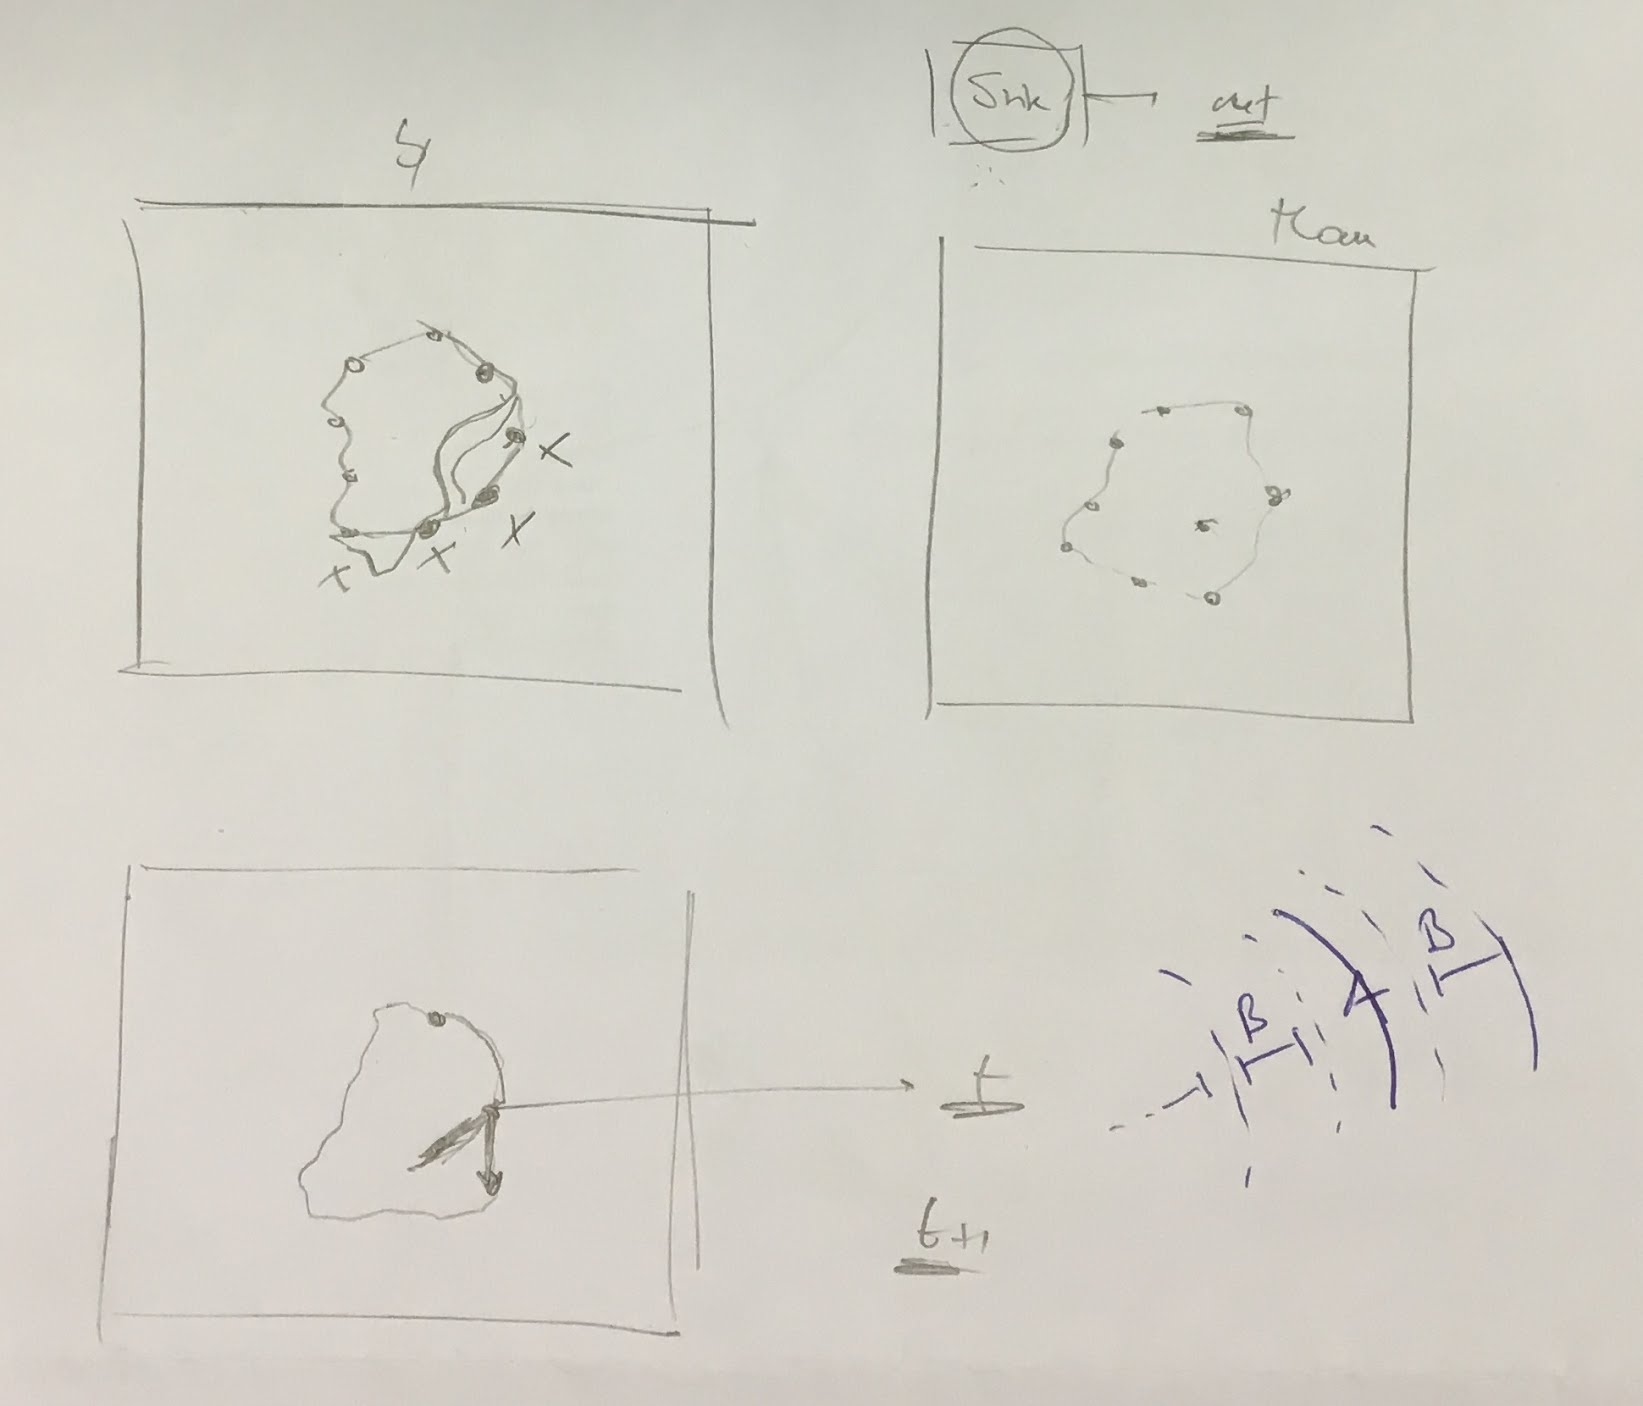
\includegraphics[width=0.60\textwidth]{annotation_predictor_2}
%\caption{Annotation Predictors Technique}
%\label{fig:annotation_predictor_2}
%\end{figure}
%
%\hfill
%
%%%%%%%%%%%%%%%%%%%%%%%%%%%%%%%%%%%%%%%%%%%%%%%%%%%%